\documentclass[a4paper, 14pt]{extarticle}
\usepackage[english,russian]{babel}
\usepackage[T1]{fontenc}
\usepackage[utf8]{inputenc}
\usepackage{fontspec}
\usepackage{indentfirst}
\usepackage{enumitem}
\usepackage{graphicx}
\usepackage[
  left=20mm,
  right=10mm,
  top=20mm,
  bottom=20mm
]{geometry}
\usepackage{parskip}
\usepackage{titlesec}
\usepackage{xurl}
\usepackage{hyperref}
\usepackage{float}
\usepackage[
  figurename=Рисунок,
  labelsep=endash,
  justification=centering
]{caption}
\usepackage[outputdir=build, newfloat]{minted}
\usepackage{chngcntr}

\selectlanguage{russian}

\hypersetup{
  colorlinks=true,
  linkcolor=black,
  filecolor=blue,
  urlcolor=blue,
}

\renewcommand*{\labelitemi}{---}
\setmainfont{Times New Roman}
\setmonofont{JetBrains Mono}[
  SizeFeatures={Size=11},
]

\newenvironment{code}{\captionsetup{type=figure}}{}
\BeforeBeginEnvironment{code}{\bigskip}
\AfterEndEnvironment{code}{\bigskip}

\setminted{
  fontsize=\footnotesize,
}

\setlength{\parskip}{6pt}

\setlength{\parindent}{1.25cm}
\setlist[itemize]{itemsep=0em,topsep=0em,parsep=0em,partopsep=0em,leftmargin=2.0cm,wide}
\setlist[enumerate]{itemsep=0em,topsep=0em,parsep=0em,partopsep=0em,leftmargin=2.0cm,wide}

\renewcommand{\thesection}{\indent\arabic{section}.}
\renewcommand{\thesubsection}{\indent\thesection\arabic{subsection}.}
\renewcommand{\thesubsubsection}{\indent\thesubsection\arabic{subsubsection}.}

\titleformat{\section}{\normalfont\bfseries}{\thesection}{0.5em}{}
\titleformat{\subsection}{\normalfont\bfseries}{\thesubsection}{0.5em}{}
\titleformat{\subsubsection}{\normalfont\bfseries}{\thesubsubsection}{0.5em}{}

\titleformat*{\section}{\normalfont\bfseries}
\titleformat*{\subsection}{\normalfont\bfseries}
\titleformat*{\subsubsection}{\normalfont\bfseries}

\titlespacing{\section}{\parindent}{\parskip}{\parskip}
\titlespacing{\subsection}{\parindent}{\parskip}{\parskip}
\titlespacing{\subsubsection}{\parindent}{\parskip}{\parskip}

\linespread{1.5}
\renewcommand{\baselinestretch}{1.5}

\begin{document}

\begin{titlepage}
  \vspace{0pt plus2fill}
  \noindent

  \vspace{0pt plus6fill}
  \begin{center}
    Санкт-Петербургский национальный исследовательский университет
    информационных технологий, механики и оптики

    \vspace{0pt plus3fill}

    Факультет инфокоммуникационных технологий

    Направление подготовки 11.03.02

    \vspace{0pt plus2fill}

    Лабораторная работа №3

    <<Идентификаторы, переменные, типы данных>>

  \end{center}

  \vspace{0pt plus6fill}
  \begin{flushright}
    Выполнил: \\
    Швалов Даниил Андреевич

    Группа: К33211

    Проверил: \\
    Иванов Сергей Евгеньевич
  \end{flushright}

  \vspace{0pt plus5fill}
  \begin{center}
    Санкт-Петербург

    2024
  \end{center}
\end{titlepage}

\setcounter{page}{2}

\section*{Введение}

Цель работы:
\begin{itemize}
  \item создание приложений, использующих встроенные типы данных и литералы
  различных типов;
  \item создание приложений, демонстрирующих возможность работы с символами
  Unicode, использование символов Unicode в составе идентификаторов.
\end{itemize}

\section*{Ход работы}

\subsection*{Задание 1. Использование встроенных типов}

В данном задании необходимо реализовать программу, которая считывает из
стандартного ввода три стороны треугольника, после чего находит по этим сторонам
площадь треугольника и выводит ее в стандартный вывод.

Для нахождения площади треугольника по трем сторонам использовалась формула
Герона, которая выглядит следующим образом:
\[
  S = \sqrt{p (p - a1) (p - a2) (p - a3)},
\]
где \(p\) --- полупериметр, \(a1\), \(a2\) и \(a3\) --- стороны треугольника.
Использование данной формулы в исходном коде было вынесено в отдельную функцию
\textit{findSquare}.

Считывание сторон треугольника было реализовано с помощью класса
\textit{Scanner} из стандартной библиотеки Java. При получении некорректных
аргументов программа завершает свое выполнение с сообщением об ошибке.

На рисунке \ref{fig:task-1} представлен пример работы программы: при вводе трех
сторон треугольника (на рисунке 3, 4 и 5) программа вывела верное значение
площади треугольника, т. е. 6.

\begin{figure}[H]
  \centering
  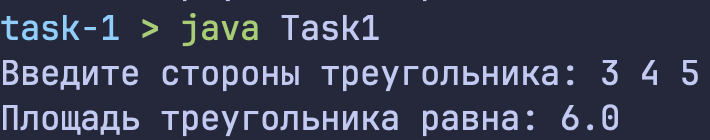
\includegraphics[width=0.6\textwidth]{images/task-1.png}
  \caption{Пример работы программы}
  \label{fig:task-1}
\end{figure}

\subsection*{Задание 2. Реализация форматированного вывода}

В данном задании необходимо использовать функции форматирования строк для вывода
результатов. Поэтому исходный код был изменен следующим образом. Вместо
использования функции \textit{println} была использована функция
\textit{printf}, которой были переданы параметры для форматирования чисел с
плавающей запятой.

В качестве формата вывода чисел с плавающей запятой был выбран формат с выводом
двух первых знаков числа после запятой. Для этого использовался параметр
\textit{\%.2f} в форматируемой строке.

На рисунке \ref{fig:task-2} представлен пример работы программы. Теперь при
выводе, кроме результата, также пишутся и стороны, переданные пользователем. Как
видно, все числа представлены с двумя знаками после запятой.

\begin{figure}[H]
  \centering
  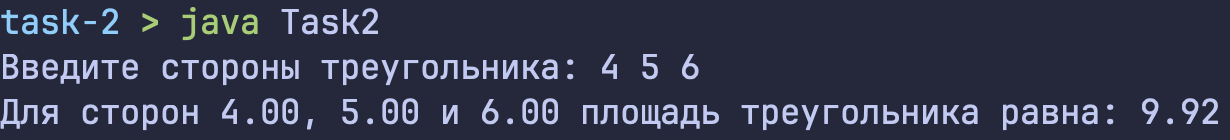
\includegraphics[width=0.8\textwidth]{images/task-2.png}
  \caption{Пример работы программы}
  \label{fig:task-2}
\end{figure}

\subsection*{Задание 3. Использование символов Unicode}

В ранее приведенных программах уже были поддержаны символы Unicode. Это,
например, было продемонстрировано при выводе кириллических символов в
стандартный вывод. Поэтому вносить дополнительных изменений в исходные коды
программ не пришлось.

\section*{Заключение}

В данной лабораторной работе было разработано приложение, которое использует
стандартные средства Java для работы с вводом выводом. При выполнении
лабораторной работы были использованы такие инструменты как класс для считывания
данных \textit{Scanner}, а также функция \textit{printf} для вывода
форматированных строк.

Цель, поставленная в начале работы, достигнута, задачи выполнены.

\end{document}
